\section{Reproducing and auditing a scalar SVE symmetry calculation}
\label{sec:sve-repro}
This section reconstructs the calculation of Paliathanasis, Leon and
Leach~\cite{ap} from the scalar equation itself. The order of the argument is
important: expand the equation, derive its infinitesimal symmetries, find
invariant graphs, and only then solve and check the resulting profile
equations. Each step supplies the input needed by the next one. The
worked Boussinesq analysis of Bruz\'{o}n and Gandarias~\cite[Sec.~2, pp.~157--159]{bruzon-gandarias-2021}
provides a useful expository model for this progression from prolongation
and determining equations to reductions and conservation laws. Its
Boussinesq-specific generators and conservation laws are not assumed for SVE.

Our target is the source's \emph{printed scalar equation}. It is distinct
from the advectively corrected scalar equation and from the full coupled
Saint--Venant--Exner system discussed in the coordinate audit~\eqref{eq:physical-bed-audit}.
We take $g,\kappa>0$, $\beta=m\kappa$, and $m\geq1$. Unless an exceptional
case is explicitly identified, the local calculation uses
\begin{equation}
 p:=\phi_t>0,\qquad q:=\phi_s>0.
 \label{eq:sve-repro-chart}
\end{equation}
The second inequality makes the material-to-position map locally invertible;
the first selects a real smooth branch of $p^{m-1}$ even when $m$ is not an
integer. A conclusion on this chart is not a conclusion at its boundary.
Numbers such as ``case 3.4'' and ``source (24)'' refer to the source paper's
subsections and equations; our own equations have the numbering of this manuscript.

\subsection{The master equation and its differentiation}
The independent variables are time $t$ and a material label $s$, and
$\phi(t,s)$ is the dependent variable. To make the differentiation explicit,
write the two currents as
\begin{equation}
 \mathcal A=q\phi_{tt}-g\frac{\phi_{ss}}{q^2},\qquad
 \mathcal J=m\kappa\frac{p^{m-1}\phi_{ts}}{q},\qquad
 E_m:=D_t\mathcal A-gD_s\mathcal J=0.
 \label{eq:sve-repro-currents}
\end{equation}
This scalar equation expresses compatibility of the source's printed
momentum and bed equations. If $\mathfrak b$ denotes its bed variable,
those equations prescribe $\mathfrak b_s=-\mathcal A/g$ and
$\mathfrak b_t=-\mathcal J$. Commuting the two mixed derivatives gives
$-D_t\mathcal A/g=-D_s\mathcal J$, which is exactly
\eqref{eq:sve-repro-currents}. The notation $\mathfrak b$ distinguishes
bed elevation from the mixed derivative $b$ introduced below. This step
uses the printed pair; it does not remove the advective discrepancy in
the physical-coordinate audit.
Here $D_t,D_s$ are total derivatives: they differentiate both explicit
coordinate dependence and every derivative of $\phi$ occurring in an
expression. Introduce the derivative coordinates
\[
 a=\phi_{tt},\quad b=\phi_{ts},\quad c=\phi_{ss},\qquad
 r=\phi_{ttt},\quad w=\phi_{tts},\quad x=\phi_{tss},\quad y=\phi_{sss}.
\]
In this subsection $x$ is a third derivative, not the Eulerian position.
For expressions through second order, the relevant parts of the total
derivative operators are
\begin{align}
 D_t&=\partial_t+p\partial_\phi+a\partial_p+b\partial_q
                 +r\partial_a+w\partial_b+x\partial_c+\cdots,\notag\\
 D_s&=\partial_s+q\partial_\phi+b\partial_p+c\partial_q
                 +w\partial_a+x\partial_b+y\partial_c+\cdots.
 \label{eq:sve-total-operators}
\end{align}
For example, $D_tq=b$, $D_tc=x$, $D_sp=b$, and $D_sb=x$.
Thus the product and quotient rules give, term by term,
\begin{align}
 D_t(qa)&=(D_tq)a+qD_ta=ab+qr,\notag\\
 D_t(cq^{-2})&=(D_tc)q^{-2}-2cq^{-3}D_tq
                =\frac{x}{q^2}-\frac{2cb}{q^3},\notag\\
 D_s(p^{m-1}bq^{-1})
   &=(m-1)p^{m-2}(D_sp)bq^{-1}
       +p^{m-1}(D_sb)q^{-1}-p^{m-1}bq^{-2}D_sq\notag\\
   &=(m-1)p^{m-2}\frac{b^2}{q}
       +p^{m-1}\frac{x}{q}-p^{m-1}\frac{bc}{q^2}.
 \label{eq:sve-current-differentiation}
\end{align}
Substitution into~\eqref{eq:sve-repro-currents} produces the expanded master
equation
\begin{align}
 E_m={}&qr+ab-g\frac{x}{q^2}+2g\frac{cb}{q^3}\notag\\
 &-gm\kappa\left((m-1)p^{m-2}\frac{b^2}{q}
       +p^{m-1}\frac{x}{q}-p^{m-1}\frac{bc}{q^2}\right)=0.
 \label{eq:sve-repro-master}
\end{align}
The coefficient of $r$ is $q$. Therefore, on the declared chart, we may solve
for precisely this derivative:
\begin{equation}
 r=\mathcal N:=-\frac{ab}{q}+\frac{gx}{q^3}-\frac{2gcb}{q^4}
 +gm\kappa\left((m-1)p^{m-2}\frac{b^2}{q^2}
              +p^{m-1}\frac{x}{q^2}-p^{m-1}\frac{bc}{q^3}\right).
 \label{eq:sve-master-normal}
\end{equation}
The remaining derivative coordinates are free coordinates of the
third-order equation manifold. Requiring an identity there permits their
coefficients to be split. It does not permit division at $q=0$, or assert
global well-posedness of the PDE.

\subsection{Infinitesimal transformations, the characteristic, and prolongation}
Begin with a near-identity point transformation, without guessing its
coefficient functions:
\begin{equation}
 \widetilde t=t+\varepsilon\tau(t,s,\phi)+O(\varepsilon^2),\quad
 \widetilde s=s+\varepsilon\xi(t,s,\phi)+O(\varepsilon^2),\quad
 \widetilde\phi=\phi+\varepsilon\eta(t,s,\phi)+O(\varepsilon^2).
 \label{eq:sve-small-transformation}
\end{equation}
Its infinitesimal generator is
\[
 X=\tau\partial_t+\xi\partial_s+\eta\partial_\phi.
\]
To see where the characteristic comes from, let $\phi=f(t,s)$ be one
particular graph. After transformation, its points obey
\[
 \widetilde f(t+\varepsilon\tau,s+\varepsilon\xi)
       =f(t,s)+\varepsilon\eta+O(\varepsilon^2),
\]
where the coefficients are evaluated at $(t,s,f(t,s))$. Write
$\widetilde f=f+\varepsilon\delta f+O(\varepsilon^2)$ and expand the
left-hand side at the \emph{same} original base point. The coefficient of
$\varepsilon$ is $\delta f+\tau f_t+\xi f_s$. Consequently
\begin{equation}
 \delta f=\eta-\tau f_t-\xi f_s,
 \qquad Q:=\eta-\tau\phi_t-\xi\phi_s.
 \label{eq:sve-characteristic-derived}
\end{equation}
Thus $Q$ measures the change in the graph after the displacement of its
independent variables has been taken into account. A graph is invariant
under the local flow when $Q[f]=0$. An \emph{equation symmetry} has a
different requirement: it maps every local solution to another solution,
which need not be the same graph.

The PDE contains derivatives, so the transformation must also act on them.
For instance, differentiating the transformed graph relation gives
\[
 D_t\widetilde\phi
   =\widetilde\phi_{\widetilde t}D_t\widetilde t
       +\widetilde\phi_{\widetilde s}D_t\widetilde s.
\]
Comparison of the first-order terms in $\varepsilon$ yields
$\widetilde\phi_{\widetilde t}=p+\varepsilon\eta^t+O(\varepsilon^2)$,
where
\begin{align}
 \eta^t&=D_t\eta-pD_t\tau-qD_t\xi
       =\eta_t+\eta_\phi p-p(\tau_t+\tau_\phi p)
                              -q(\xi_t+\xi_\phi p),\notag\\
 \eta^s&=D_s\eta-pD_s\tau-qD_s\xi
       =\eta_s+\eta_\phi q-p(\tau_s+\tau_\phi q)
                              -q(\xi_s+\xi_\phi q).
 \label{eq:sve-first-prolongation}
\end{align}
Superscripts here label transformed derivative coefficients; $\eta^t$ is
not the ordinary partial derivative $\eta_t$. Applying the same chain rule
again gives, for any derivative multi-index $I$,
\begin{equation}
 \eta^{Ii}=D_i\eta^I-\phi_{It}D_i\tau-\phi_{Is}D_i\xi,
 \qquad i\in\{t,s\},\qquad \eta^\varnothing=\eta.
 \label{eq:sve-prolongation-recursion}
\end{equation}
For clarity, the second-order coefficients and the third-order ones needed
by the master equation are
\begin{align}
 \eta^{tt}&=D_t^2\eta-pD_t^2\tau-qD_t^2\xi
                          -2aD_t\tau-2bD_t\xi,\notag\\
 \eta^{ts}&=D_tD_s\eta-pD_tD_s\tau-qD_tD_s\xi
                    -aD_s\tau-bD_s\xi-bD_t\tau-cD_t\xi,\notag\\
 \eta^{ss}&=D_s^2\eta-pD_s^2\tau-qD_s^2\xi
                          -2bD_s\tau-2cD_s\xi,\notag\\
 \eta^{ttt}&=D_t\eta^{tt}-rD_t\tau-wD_t\xi,\notag\\
 \eta^{tss}&=D_t\eta^{ss}-xD_t\tau-yD_t\xi.
 \label{eq:sve-higher-prolongation}
\end{align}
These formulas specify a finite symbolic calculation, rather than an
unspecified appeal to prolongation. The infinitesimal criterion
\cite{olver,oliveri2026} is
\begin{equation}
 \Omega:=\left.\pr^{(3)}X(E_m)\right|_{r=\mathcal N}=0,
 \label{eq:sve-omega}
\end{equation}
as an identity in all the remaining free derivative coordinates.

Since the expanded $E_m$ has no explicit $t,s,\phi,w,y$ dependence, the
expression to be calculated before restriction is exactly
\begin{equation}
 \pr^{(3)}X(E_m)=\eta^t E_p+\eta^s E_q+\eta^{tt}E_a
       +\eta^{ts}E_b+\eta^{ss}E_c+\eta^{ttt}E_r+\eta^{tss}E_x.
 \label{eq:sve-prolonged-master}
\end{equation}
Its partial derivatives, obtained directly from
\eqref{eq:sve-repro-master}, are
\begin{align}
 E_p={}&-gm\kappa(m-1)\left((m-2)p^{m-3}\frac{b^2}{q}
               +p^{m-2}\frac{x}{q}-p^{m-2}\frac{bc}{q^2}\right),\notag\\
 E_q={}&r+\frac{2gx}{q^3}-\frac{6gcb}{q^4}
       +gm\kappa\left((m-1)p^{m-2}\frac{b^2}{q^2}
           +p^{m-1}\frac{x}{q^2}-2p^{m-1}\frac{bc}{q^3}\right),\notag\\
 E_a={}&b,\qquad
 E_b=a+\frac{2gc}{q^3}-\frac{2gm\kappa(m-1)p^{m-2}b}{q}
                         +\frac{gm\kappa p^{m-1}c}{q^2},\notag\\
 E_c={}&\frac{2gb}{q^3}+\frac{gm\kappa p^{m-1}b}{q^2},\qquad
 E_r=q,\qquad E_x=-\frac{g}{q^2}-\frac{gm\kappa p^{m-1}}q.
 \label{eq:sve-master-partials}
\end{align}
The free coordinates $w,y$ can still occur in~\eqref{eq:sve-prolonged-master}
through the prolonged coefficients. This explains why their coefficients
give useful determining equations even though $E_m$ itself has no $w,y$ terms.

\subsection{Determining equations and the parameter-dependent point algebras}
We now solve~\eqref{eq:sve-omega} in stages. Every displayed coefficient
below is taken \emph{after} the restrictions obtained in preceding stages;
the notation $[y]\Omega$ means the coefficient of the free coordinate $y$.
\begin{enumerate}
\item The coefficient of $y$ is
\[
 [y]\Omega=\frac{g(\kappa mp^mq+p)}{pq^2}(\xi_t+p\xi_\phi).
\]
Its prefactor is strictly positive on~\eqref{eq:sve-repro-chart}.
For fixed $(t,s,\phi)$, the identity $\xi_t+p\xi_\phi=0$ holds for
every $p>0$, not one chosen velocity. Differentiation with respect to this
free $p$ gives $\xi_\phi=0$, and substitution gives $\xi_t=0$.
Thus $\xi=\xi(s)$.
\item With this restriction, the coefficient of $w$ becomes
\[
 [w]\Omega=\frac{2g(\kappa mp^mq+p)}{pq^2}(\tau_s+q\tau_\phi).
\]
Varying the independent free coordinate $q>0$ gives $\tau_\phi=0$
and then $\tau_s=0$. Hence $\tau=\tau(t)$.
\item The coefficient of the product $ab$ is now $-\eta_s/q$.
It must vanish, so $\eta_s=0$ and $\eta=\eta(t,\phi)$.
\item The coefficient of $a$ is then
\begin{equation}
 [a]\Omega=q(4p\eta_{\phi\phi}-3\tau''+4\eta_{t\phi}).
 \label{eq:sve-repro-split}
\end{equation}
Splitting in $p$ gives $\eta_{\phi\phi}=0$ and
$4\eta_{t\phi}=3\tau''$. Integrating the former with respect to
$\phi$ gives $\eta=A(t)\phi+B(t)$; the latter becomes $4A'=3\tau''$.
In particular, the affine dependence on $\phi$ has been derived, not assumed.
\item Finally the coefficient of $x$ is
\begin{align}
 [x]\Omega=-\frac{g}{p^2q^2}\big\{&\kappa mp^mq
     [(m-3)p(A-\tau')+(m-1)(A'\phi+B')]\notag\\
     &+p^2(2\tau'+\xi'-3A)\big\}.
 \label{eq:sve-repro-xsplit}
\end{align}
Multiplication by $-p^2q^2/g$ is allowed on the chart. The result is
affine in the free $q$, so its constant and linear coefficients must
vanish separately. We obtain
\begin{align}
 2\tau'+\xi'-3A&=0, &4A'&=3\tau'',\notag\\
 (m-3)(A-\tau')&=0,&(m-1)A'&=0,&(m-1)B'&=0.
 \label{eq:sve-final-determining}
\end{align}
The second line follows by varying $p$ and $\phi$ independently in the
square bracket of~\eqref{eq:sve-repro-xsplit}.
\end{enumerate}
We must separate $m=1$ and $m=3$ before dividing by the factors $m-1$ or
$m-3$. Integration of~\eqref{eq:sve-final-determining} gives the following.
\begin{description}
\item[Generic stratum, $m\ne1,3$.]
Here $A=\tau'$, $A'=B'=0$, and $\xi'=A$. Thus, for constants
$c_t,c_s,c_\phi,d$,
\[
 \tau=c_t+dt,\qquad \xi=c_s+ds,\qquad \eta=c_\phi+d\phi.
\]
\item[Cubic stratum, $m=3$.]
Here $A'=B'=0$, whence $\tau''=0$. Writing $A=d$ and $\tau'=e$
gives
\[
 \tau=c_t+et,\qquad \xi=c_s+(3d-2e)s,\qquad \eta=c_\phi+d\phi.
\]
The scaling part is $dX_4+(e-d)X_5$ in the basis below.
\item[Linear-flux stratum, $m=1$.]
The equations give $A=\tau'$, while $4A'=3\tau''$ then forces
$A'=\tau''=0$; also $\xi'=A$. At this stage $B(t)$ is still arbitrary.
Substitution of these functions into the \emph{full} prolonged equation,
not just its selected coefficients, gives
\[
 \pr^{(3)}X(E_1)+2A E_1=bB''+qB'''.
\]
The independent coefficient of $b$ therefore requires $B''=0$.
Consequently $B=c_\phi+vt$ and
\[
 \tau=c_t+dt,\qquad \xi=c_s+ds,\qquad
 \eta=c_\phi+d\phi+vt.
\]
\end{description}

\begin{table}[htbp]
\centering\small
\begin{tabularx}{\linewidth}{@{}lXll@{}}
\toprule
Field & Explicit infinitesimal generator & Admitted parameters & Flow $(\widetilde t,\widetilde s,\widetilde\phi)$\\
\midrule
$X_1$ & $\partial_t$ & all $m\geq1$ & $(t+\varepsilon,s,\phi)$\\
$X_2$ & $\partial_s$ & all $m\geq1$ & $(t,s+\varepsilon,\phi)$\\
$X_3$ & $\partial_\phi$ & all $m\geq1$ & $(t,s,\phi+\varepsilon)$\\
$X_4$ & $t\partial_t+s\partial_s+\phi\partial_\phi$ & all $m\geq1$ & $(e^\varepsilon t,e^\varepsilon s,e^\varepsilon\phi)$\\
$X_5$ & $t\partial_t-2s\partial_s$ & $m=3$ & $(e^\varepsilon t,e^{-2\varepsilon}s,\phi)$\\
$X_6$ & $t\partial_\phi$ & $m=1$ & $(t,s,\phi+\varepsilon t)$\\
\bottomrule
\end{tabularx}
\caption{Listed Lie symmetries, including the additional $m=1$ generator.
The flows solve $d\widetilde t/d\varepsilon=\tau$,
$d\widetilde s/d\varepsilon=\xi$, $d\widetilde\phi/d\varepsilon=\eta$
with the identity initial condition at $\varepsilon=0$.}
\label{tab:sve-generators}
\end{table}

Necessity is only half of the classification argument. Direct substitution
of the resulting fields into~\eqref{eq:sve-prolonged-master} verifies
\begin{align}
 \pr^{(3)}X_i(E_m)&=0\quad(i=1,2,3),&
 \pr^{(3)}X_4(E_m)&=-2E_m,\notag\\
 \pr^{(3)}X_5(E_m)+E_m&=(3-m)E_{\rm bed},&
 E_{\rm bed}&=-gm\kappa D_s(p^{m-1}b/q),\notag\\
 \pr^{(3)}X_6(E_1)&=0.
 \label{eq:sve-offshell-certificates}
\end{align}
An equality such as $\pr^{(3)}X_4(E_m)=-2E_m$ is sufficient because its
right-hand side vanishes whenever $E_m=0$; off-shell zero is not required.
For an additional check, under $X_4$, $p,q$ have weight zero, $a,b,c$
weight $-1$, and $r,w,x,y$ weight $-2$. Every term of the master equation
has weight $-2$, explaining that multiplier. Under $X_5$, the inertial
and gravity part has weight $-1$ and $E_{\rm bed}$ weight $2-m$,
which gives the second identity. At $m=1$ the equation has no explicit
dependence on $p$; the boost $\phi\mapsto\phi+\varepsilon t$ changes
only $p$ among its derivative arguments.

\begin{proposition}[Local smooth point classification on the positive chart]
For the printed scalar equation, fixed $g,\kappa>0$ and $m\geq1$, the local
smooth point algebra on $p,q>0$ has basis $X_1,\ldots,X_4$ for $m\ne1,3$,
basis $X_1,\ldots,X_5$ for $m=3$, and basis $X_1,X_2,X_3,X_4,X_6$ for
$m=1$. Its dimensions are therefore $4,5,5$, respectively.
\end{proposition}
The coefficient argument exhausts the unrestricted smooth functions
$\tau,\xi,\eta$; the off-shell identities prove sufficiency. This is
stronger than checking a finite guessed list, but its scope remains local
point transformations on the stated chart. It does not classify generalized
symmetries, the boundary $p=0$, or the full bed-field system.
The source lists the four common generators and the cubic extension but
omits the $m=1$ boost. Moreover, its printed determining condition
$3\eta^1+\xi^2_{,s}+2\xi^1_{,t}=0$ gives $6=0$ on its own $X_4$.
That determining condition is inconsistent, although the generator itself
passes the independent calculation above.

\subsection{Commutators, adjoint actions, and a one-dimensional optimal system}
For coordinate fields $U=U^j\partial_j$, $V=V^j\partial_j$, our convention is
\begin{equation}
 [U,V]=\sum_j\left(\sum_i U^i\partial_iV^j
                          -V^i\partial_iU^j\right)\partial_j.
 \label{eq:sve-bracket-rule}
\end{equation}
For example, $\partial_t$ differentiates the $t$ coefficient of $X_4$,
so $[X_1,X_4]=\partial_t=X_1$. Similarly,
$[X_2,X_5]=\partial_s(-2s)\partial_s=-2X_2$.
The entire cubic commutator table is consequently
Table~\ref{tab:sve-repro-brackets}; its upper-left block gives the generic
algebra. At $m=1$ use $X_6$ instead of $X_5$, with the additional nonzero
pair $[X_1,X_6]=X_3$, $[X_6,X_1]=-X_3$; all its other brackets with
$X_2,X_3,X_4$ vanish.
\begin{table}[htbp]
\centering\small
\begin{tabular}{@{}c|ccccc@{}}
\toprule
$[\text{row},\text{column}]$ & $X_1$ & $X_2$ & $X_3$ & $X_4$ & $X_5$\\
\midrule
$X_1$ & $0$ & $0$ & $0$ & $X_1$ & $X_1$\\
$X_2$ & $0$ & $0$ & $0$ & $X_2$ & $-2X_2$\\
$X_3$ & $0$ & $0$ & $0$ & $X_3$ & $0$\\
$X_4$ & $-X_1$ & $-X_2$ & $-X_3$ & $0$ & $0$\\
$X_5$ & $-X_1$ & $2X_2$ & $0$ & $0$ & $0$\\
\bottomrule
\end{tabular}
\caption{Commutators of the admitted Lie symmetries at $m=3$.
The last-row entries correct two reverse-order signs in source Table 1.}
\label{tab:sve-repro-brackets}
\end{table}

One-dimensional subalgebras generated by $X$ and $cX$, $c\ne0$, are the
same line. A symmetry of the equation may also conjugate one line to
another. An optimal system chooses one representative from each such
equivalence class, avoiding repeated reductions. Here the equivalence is
\emph{connected inner adjoints and nonzero real line rescaling}; outer or
discrete automorphisms are not silently included. With the source's sign
convention the adjoint series is
\begin{equation}
 \operatorname{Ad}(e^{\varepsilon U})V
 =e^{-\varepsilon\operatorname{ad}_U}V
 =V-\varepsilon[U,V]+\frac{\varepsilon^2}{2}[U,[U,V]]-\cdots.
 \label{eq:sve-adjoint-series}
\end{equation}
For example,
$\operatorname{Ad}(e^{\varepsilon X_1})X_4=X_4-\varepsilon X_1$,
whereas $[X_4,X_1]=-X_1$ gives
$\operatorname{Ad}(e^{\varepsilon X_4})X_1=e^\varepsilon X_1$.
These two calculations explain translation removal and positive scaling,
the two operations used below. All 25 entries of the source's Table 2
agree with this convention when calculated from the corrected brackets.

For generic $m$, write $Z=v_1X_1+v_2X_2+v_3X_3+hX_4$.
If $h\ne0$, an $X_i$ adjoint sends $v_i$ to $v_i-\varepsilon h$;
choosing $\varepsilon=v_i/h$ removes that component. Line rescaling then
leaves $X_4$. If $h=0$, the only nontrivial adjoint rescales all three
$v_i$ by the same positive factor. Thus the translation lines form
$\mathbb{RP}^2$, with the three disjoint coordinate charts shown in
Table~\ref{tab:sve-optimal-generic}. In particular, $X_2+X_3$ cannot
be changed into a pure translation or into a line with a nonzero $X_1$
component. This gives a concrete omission from the printed optimal list.
\begin{table}[htbp]
\centering\small
\begin{tabular}{@{}lll@{}}
\toprule
Coefficient condition & Representative & Free parameters\\
\midrule
$h\ne0$ & $\langle X_4\rangle$ & none\\
$h=0,\ v_1\ne0$ & $\langle X_1+aX_2+bX_3\rangle$ & $a,b\in\mathbb R$\\
$h=v_1=0,\ v_2\ne0$ & $\langle X_2+aX_3\rangle$ & $a\in\mathbb R$\\
$h=v_1=v_2=0$ & $\langle X_3\rangle$ & $v_3\ne0$\\
\bottomrule
\end{tabular}
\caption{One-dimensional optimal system for $m\ne1,3$ under the declared equivalence.}
\label{tab:sve-optimal-generic}
\end{table}

At $m=3$, put $Z=v_1X_1+v_2X_2+v_3X_3+\mathcal H$ with
$\mathcal H=aX_4+bX_5$. The three weights of
$\operatorname{ad}_{\mathcal H}$ on translations are
$-(a+b)$, $-(a-2b)$ and $-a$. An $X_i$ adjoint therefore removes
$v_i$ exactly when its corresponding weight is nonzero. The direction
$(a:b)$ cannot be changed by an inner adjoint. There are three exceptional
directions where a translation survives:
\[
 X_5+cX_3,\qquad X_4-X_5+cX_1,\qquad
 X_4+\tfrac12X_5+cX_2.
\]
For a nonzero survivor, a complementary dilation normalizes its magnitude
to one; its sign remains. The case $c=0$ is already the pure dilation.
When $a=b=0$, the exact translation equivalence is
\begin{equation}
 (v_1,v_2,v_3)\sim\lambda(e^\varepsilon v_1,e^{-2\varepsilon}v_2,v_3),
 \qquad \lambda\ne0,\quad\varepsilon\in\mathbb R.
 \label{eq:sve-translation-orbits}
\end{equation}
It preserves the support and relative signs. For $v_3\ne0$ it also
preserves $v_1^2v_2/v_3^3$, as direct cancellation of the factors shows.
Disjoint representatives for pure translations are
\[
 \begin{gathered}
 X_1,\ X_2,\ X_3;\qquad X_1\pm X_2,\quad X_3\pm X_1,\quad X_3\pm X_2;\\
 X_3+\sigma X_1+KX_2,\qquad \sigma\in\{-1,1\},\quad K\ne0.
 \end{gathered}
\]
In the last family $K=v_1^2v_2/v_3^3$. Together with all projective
dilation directions and their resonant survivors, these describe the
cubic line orbits.

At $m=1$, write instead $Z=v_1X_1+v_2X_2+v_3X_3+hX_4+cX_6$.
The $X_6$ adjoint changes $v_3$ to $v_3+\varepsilon v_1$, and the
$X_1$ adjoint changes it to $v_3-\varepsilon c$. If $h\ne0$,
translations can be removed, leaving $X_4+aX_6$. If $h=0,c\ne0$,
normalize $c=1$, remove $v_3$, and use positive common scaling on
$(v_1,v_2)$. If $h=c=0$, remove $v_3$ whenever $v_1\ne0$.
The resulting disjoint families are
\[
 \begin{array}{c|l}
 h\ne0 & X_4+aX_6\\
 h=0,\ c\ne0 & X_6,\quad X_6+\sigma X_1+aX_2,\quad X_6+\sigma X_2\\
 h=c=0 & X_1+aX_2,\quad X_2+aX_3,\quad X_3
 \end{array}
 \quad(a\in\mathbb R,\ \sigma=\pm1).
\]
These are algebraic orbit classifications. The additional requirements
for an invariant graph, a regular reduced equation, and compatible data
must still be checked; the next subsection makes that distinction concrete.

\subsection{Similarity transformations and invariant graphs}
An invariant coordinate $z(t,s,\phi)$ satisfies $X(z)=0$. A second
independent invariant $W$ then allows an invariant graph to be written
as $W=F(z)$ whenever the graph projection is regular. This is the
geometric reason that one arbitrary function of two variables can be
replaced, within a symmetry-invariant subclass, by one function of one
variable. It is a restriction on solutions, not a claim that all PDE
solutions have this form.

For $X_4$, the flow in Table~\ref{tab:sve-generators} leaves $s/t$ and
$\phi/t$ unchanged on $t>0$. Hence
\[
 z=s/t,\quad W=\phi/t,\quad W=F(z)
 \quad\Longrightarrow\quad \phi=tF(s/t).
\]
One may check the same result without integrating the flow:
$X_4(s/t)=0$, $X_4(\phi/t)=0$, and
$Q=\phi-t\phi_t-s\phi_s$ vanishes on this graph.
For $X_5$, $X_5(st^2)=2st^2-2st^2=0$ and $X_5(\phi)=0$;
thus $z=st^2$, $W=\phi$, and $\phi=F(st^2)$.
For a traveling generator
$X=X_1+\alpha X_2+\alpha_3X_3$, the flow is
\[
 (t,s,\phi)\longmapsto
 (t+\varepsilon,s+\alpha\varepsilon,\phi+\alpha_3\varepsilon).
\]
It fixes $z=s-\alpha t$ and $W=\phi-\alpha_3t$, giving
$\phi=\alpha_3t+F(s-\alpha t)$. In each example the equation
$W=F(z)$ is precisely the integrated graph condition $Q=0$.

\begin{table}[htbp]
\centering\small
\begin{tabularx}{\linewidth}{@{}p{.85cm}p{2.6cm}p{2.7cm}X@{}}
\toprule
Case & Generator & Invariants $(z,W)$ & Invariant graph and outcome\\
\midrule
3.1 & $X_1$ & $(s,\phi)$ & $\phi=F(s)$; identity, outside $p>0$\\
3.2 & $X_2$ & $(t,\phi)$ & $\phi=F(t)$; $q=0$, PDE undefined\\
3.3 & $X_3$ & $(t,s)$ & $Q=1$; no invariant graph\\
3.4 & $X_4$ & $(s/t,\phi/t)$ & $\phi=tF(z)$; common-scaling ODE\\
3.5 & $X_5$, $m=3$ & $(st^2,\phi)$ & $\phi=F(z)$; cubic-scaling ODE\\
3.6 & $X_1+\alpha X_2$ & $(s-\alpha t,\phi)$ & $\phi=F(z)$; traveling ODE\\
3.7 & $X_1+\alpha X_3$ & $(s,\phi-\alpha t)$ & $\phi=\alpha t+F(s)$; identity\\
3.8 & $X_2+\alpha X_3$ & $(t,\phi-\alpha s)$ & $\phi=\alpha s+F(t)$; $\alpha F'''=0$\\
3.9 & $X_1+\alpha X_2+\alpha_3X_3$ & $(s-\alpha t,\phi-\alpha_3t)$ & $\phi=\alpha_3t+F(z)$; traveling ODE\\
\bottomrule
\end{tabularx}
\caption{Lie invariants and corrected graphs for the source's nine numbered
cases. This is the audited source selection, not a complete optimal system
for every parameter stratum. Scaling graphs use $t>0$; regular ODE
evolution additionally requires its leading coefficient to be nonzero.}
\label{tab:sve-repro-invariants}
\end{table}

The word ``Lagrangian'' needs care here. A \emph{material coordinate}
labels particles, whereas a \emph{variational Lagrangian} is an action
density $\mathcal L$ for which the Euler--Lagrange expression
\[
 \frac{\delta\mathcal L}{\delta\phi}
 =\sum_{i,j\geq0}(-D_t)^i(-D_s)^j
       \frac{\partial\mathcal L}{\partial\phi_{t^is^j}}
\]
produces the equation, possibly in a separately justified equivalent
formulation. The source reports that it could not find such a
Lagrangian; that is not a proof of nonexistence. If an action were
obtained, one would still have to verify its Euler--Lagrange equation
and determine which of the point symmetries preserve the action up to a
divergence before applying Noether's theorem~\cite{noether}.
The reductions below require no variational action. A conservation
identity can instead be verified directly, as the Boussinesq chapter
illustrates with multipliers before deriving traveling-wave first
integrals~\cite[Sec.~4, pp.~166--169]{bruzon-gandarias-2021}.

\subsection{Direct calculation of all nine reduced equations}
Write $P=F'$, $C=F''$ and $H=F'''$, where primes differentiate the
specified invariant coordinate. When $G=G(z,F,P,C)$ is an expression
on a profile, its total derivative is
\begin{equation}
 D G=G_z+PG_F+CG_P+HG_C.
 \label{eq:sve-profile-total}
\end{equation}
The derivative $G_z$ on the right is the partial derivative at fixed
$F,P,C$; the remaining terms account for their dependence on $z$.
This convention makes every current calculation below unambiguous.

\subsubsection{Translations and exceptional graph outcomes: cases 3.1--3.3, 3.7 and 3.8}
For case 3.1, $Q=-\phi_t=0$ gives $\phi=F(s)$. Then
$p=a=b=r=x=0$ and $q=F'>0$. In the current form the sediment
current is zero and $\mathcal A=-gF''/(F')^2$ is independent of $t$,
so $E_m=0$. This stationary family lies outside $p>0$; it is evaluated
as a separate current-form branch rather than by inserting $p=0$
into the differentiated real-power formula.
Case 3.2 has $Q=-\phi_s=0$, hence $q=0$, where the master currents
are undefined. Case 3.3 has $Q=1$, so it has no invariant graph at all.
The existence of two invariant base coordinates for $X_3$ does not
overcome this obstruction to a graph.

For case 3.7, $Q=\alpha-\phi_t=0$ integrates to
$\phi=\alpha t+F(s)$. Here $p=\alpha$, $q=P$, $c=C$, while
all second or higher derivatives involving $t$ vanish. Again
$\mathcal J=0$ and $D_t\mathcal A=0$. Every sufficiently smooth $F$
with $P>0$ is allowed on the positive chart if $\alpha>0$; an
identity equation cannot select a unique third-order IVP.

For case 3.8, $Q=\alpha-\phi_s=0$ instead gives
$\phi=\alpha s+F(t)$. Now
\[
 p=P,\quad q=\alpha,\quad a=C,\quad r=H,
 \qquad b=c=w=x=y=0.
\]
Thus $\mathcal A=\alpha C$, $\mathcal J=0$, and
$E_m=\alpha H$. With $\alpha>0$,
\begin{equation}
 F'''=0,\qquad F''=c_2,\qquad F'=c_1+c_2t,\qquad
 F=c_0+c_1t+\tfrac12c_2t^2.
 \label{eq:sve-quadratic-reduction}
\end{equation}
The remaining velocity condition is $c_1+c_2t>0$ on the chosen interval.
The source interchanges the graphs of 3.7 and 3.8. The distinction matters:
the arbitrary spatial profile in 3.7 is not forced to be quadratic, whereas
the temporal profile in 3.8 is. For example,
$\phi=t+s+s^3/6$ gives $p=1$, $q=1+s^2/2>0$ and $E_m=0$, although
its spatial profile has $F'''=1$.

\subsubsection{Scaling pullbacks and the common-scaling equation: case 3.4}
Both scaling examples can be calculated once with the template
\begin{equation}
 \phi=t^A F(z),\qquad z=st^B,\qquad
 V=AF+BzP,\qquad t>0.
 \label{eq:sve-repro-scale}
\end{equation}
The generator is $t\partial_t-Bs\partial_s+A\phi\partial_\phi$.
Since $z_t=Bz/t$ and $z_s=t^B$, any profile expression $G$ satisfies
\begin{equation}
 D_t(t^dG)=t^{d-1}(dG+BzDG),\qquad
 D_s(t^dG)=t^{d+B}DG.
 \label{eq:sve-scaling-chain}
\end{equation}
For example, $\phi_t=t^{A-1}V$ and $\phi_s=t^{A+B}P$.
Applying~\eqref{eq:sve-scaling-chain} repeatedly gives the complete
derivative substitution
\begin{align}
 p&=t^{A-1}V,&q&=t^{A+B}P,\notag\\
 a&=t^{A-2}a_*,&b&=t^{A+B-1}DV,&c&=t^{A+2B}C,\notag\\
 r&=t^{A-3}((A-2)a_*+BzDa_*),&
 w&=t^{A+B-2}Da_*,\notag\\
 x&=t^{A+2B-1}D^2V,&y&=t^{A+3B}H,
 \qquad a_*=(A-1)V+BzDV.
 \label{eq:sve-scaling-jets}
\end{align}
In particular the time dependence is retained; the calculation is not
only a substitution on the slice $t=1$.

The terms $qa$ and $gc/q^2$ have time exponents $2A+B-2$ and $-A$.
They match when $3A+B=2$. Meanwhile $D_s\mathcal J$ has exponent
$(m-1)(A-1)-1+B$. For it to match $D_t\mathcal A$, this exponent
must equal $-A-1$. Together the two conditions are
\[
 3A+B=2,\qquad (m-3)(A-1)=0.
\]
These are the same restrictions already supplied by the symmetry
classification. For admitted scalings define
\[
 J_A=Pa_*-gC/P^2,\qquad J_s=m\kappa V^{m-1}(DV)/P.
\]
The current derivatives then yield
\begin{equation}
 E_m[t^AF(st^B)]=t^{-A-1}\mathcal R_{A,B},\qquad
 \mathcal R_{A,B}=-A J_A+BzD J_A-gD J_s.
 \label{eq:sve-repro-scale-residual}
\end{equation}
Thus $E_m=0$ is equivalent to the single profile ODE
$\mathcal R_{A,B}=0$ on $t>0$, with $V,P>0$.

For case 3.4, $(A,B)=(1,-1)$. Successive derivatives are especially simple:
\[
 V=F-zP,\qquad DV=-zC,\qquad a_*=z^2C,
 \qquad J_A=(z^2P-g/P^2)C,\quad
 J_s=-m\kappa zV^{m-1}C/P.
\]
Because $\mathcal R_{1,-1}=-J_A-zDJ_A-gDJ_s$, the product rule
$D(zJ_A)=J_A+zDJ_A$ gives
\begin{equation}
 \mathcal R_{1,-1}=D I_4,\qquad
 I_4=K_4 C,\qquad
 K_4=-z^3P+\frac{gz}{P^2}
                 +\frac{gm\kappa z(F-zP)^{m-1}}P.
 \label{eq:sve-repro-first-integral}
\end{equation}
This explains where the integral comes from, rather than only proposing
a candidate and stating that it works. Expanding its derivative gives
the explicit third-order equation
\begin{equation}
 K_4H+\big((K_4)_z+P(K_4)_F+C(K_4)_P\big)C=0.
 \label{eq:sve-common-expanded}
\end{equation}
Integration lowers the order: $K_4F''=I_0$. On $K_4\ne0$ it is the
two-state system $F'=P$, $P'=I_0/K_4(z,F,P)$, with
$I_0=K_4(z_0,F_0,P_0)C_0$. No initial datum is discarded: the third
initial value is encoded in $I_0$.

\subsubsection{The cubic scaling and its further reduction: case 3.5}
Here $m=3$, $A=0$, $B=2$, so direct use of the same chain rule gives
\[
 V=2zP,\qquad DV=2P+2zC,\qquad a_*=2zP+4z^2C,
\]
and hence
\[
 J_A=2zP^2+(4z^2P-g/P^2)C,\qquad
 J_s=24\kappa z^2P^2+24\kappa z^3PC.
\]
Put $\chi=12g\kappa-4$. The derivatives of these two explicit
currents reduce~\eqref{eq:sve-repro-scale-residual} to
\begin{align}
 \mathcal R_{0,2}=-\frac{2z}{P^3}\big\{&
    P(\chi z^2P^3+g)H+(\chi z^2P^3-2g)C^2\notag\\
    &+(60g\kappa-12)zP^4C+(24g\kappa-2)P^5\big\}=0.
 \label{eq:sve-cubic-expanded}
\end{align}
Since $P>0$ and $V=2zP>0$, this
chart requires $z>0$. Its leading coefficient is
\[
 L_5=-2z(\chi z^2P^3+g)/P^2.
\]
One may solve for $H$ only if $L_5\ne0$.

The equation contains $P,C,H$ but not $F$. Setting $\mu=F'$ therefore
gives a second-order equation for $\mu$, obtained by replacing
$(P,C,H)$ with $(\mu,\mu',\mu'')$ in the braces of
\eqref{eq:sve-cubic-expanded}. The inherited $X_4$ scaling acts on
$(z,F)$ as $3z\partial_z+F\partial_F$: indeed $X_4(st^2)=3st^2$.
The prolongation coefficient for $\mu=F'$ is $\mu-3\mu=-2\mu$.
Thus the induced field is $3z\partial_z-2\mu\partial_\mu$.
Its invariants on the first derivative space are
\[
 \Sigma=z^{2/3}\mu,\qquad M=z^{5/3}\mu'.
\]
Their derivatives, calculated before any division, are
\[
 \frac{d\Sigma}{dz}=z^{-1}(\tfrac23\Sigma+M),\qquad
 \frac{dM}{dz}=z^{-1}(\tfrac53M+z^{8/3}\mu'').
\]
Consequently
\begin{equation}
 \frac{dM}{d\Sigma}=
 \frac{\tfrac53M+z^{8/3}\mu''}{\tfrac23\Sigma+M}.
 \label{eq:sve-repro-mu}
\end{equation}
To make the last reduction explicit, substitution of
$\mu=\Sigma z^{-2/3}$ and $\mu'=Mz^{-5/3}$ into the second-order
equation gives
\[
 z^{8/3}\mu''=-\frac{N(\Sigma,M)}{\Sigma(\chi\Sigma^3+g)},
\]
where
\[
 N(\Sigma,M)=(\chi\Sigma^3-2g)M^2
       +(60g\kappa-12)\Sigma^4M+(24g\kappa-2)\Sigma^5.
\]
The corrected first-order equation is therefore
\begin{equation}
 \frac{dM}{d\Sigma}=
 \frac{\tfrac53M-N(\Sigma,M)/[\Sigma(\chi\Sigma^3+g)]}
      {\tfrac23\Sigma+M}.
 \label{eq:sve-cubic-first-order}
\end{equation}
Its additional chart conditions are $\Sigma>0$,
$\chi\Sigma^3+g\ne0$ and $\tfrac23\Sigma+M\ne0$.
If the last factor vanishes, $\Sigma$ is not a valid new independent
variable there; this does not establish nonexistence of a solution in the
original variables. Source (27) misses this chain-rule denominator.
Calling an equation ``Abel-type'' is not a substitute for specifying the
equation and the chart on which it was obtained.

The source also lists the mixed cubic generator $X_4+\lambda X_5$.
When $\lambda\ne-1$, division by its nonzero time coefficient gives
$A=1/(1+\lambda)$ and $B=(2\lambda-1)/(1+\lambda)$ in the preceding
template. At $\lambda=-1$, one instead has
$X_4-X_5=3s\partial_s+\phi\partial_\phi$. Its invariants on $s>0$
are $t$ and $\phi s^{-1/3}$, so the graph is $\phi=s^{1/3}F(t)$.
This is a separate coordinate chart, not a permissible substitution into
a formula divided by $1+\lambda$. The mixed family is a companion to the
nine numbered source cases, rather than an extra numerical campaign here.

\subsubsection{Traveling graphs, first integrals, and quadratures: cases 3.6 and 3.9}

Let $z=s-\alpha t$, $\phi=\alpha_3t+F(z)$, and
$v=\alpha_3-\alpha P$; case 3.6 has $\alpha_3=0$.
The chain rule gives every derivative needed by the original equation:
\begin{align}
 p&=v,&q&=P,&a&=\alpha^2C,&b&=-\alpha C,&c&=C,\notag\\
 r&=-\alpha^3H,&w&=\alpha^2H,&x&=-\alpha H,&y&=H.
 \label{eq:sve-travel-jets}
\end{align}
On profile functions, $D_t=-\alpha D$ and $D_s=D$. The two currents
are therefore
\[
 \mathcal A=(\alpha^2P-g/P^2)C,\qquad
 \mathcal J=-\alpha m\kappa v^{m-1}C/P.
\]
Inserting them into the current equation and factoring the common
constant $-\alpha$ gives, without division,
\begin{equation}
 E_m=-\alpha D\{B(P)C\},\qquad
 B(P)=\alpha^2P-\frac g{P^2}-\frac{gm\kappa v^{m-1}}P.
 \label{eq:sve-repro-travel}
\end{equation}
Here $B(P)$ is a function of the slope, distinct from the scaling exponent
$B$ of the previous subsection. Its derivative with respect to $P$ is
\begin{equation}
 B'(P)=\alpha^2+\frac{2g}{P^3}
    +gm\kappa\left(\frac{\alpha(m-1)v^{m-2}}P
                         +\frac{v^{m-1}}{P^2}\right).
 \label{eq:sve-travel-Bprime}
\end{equation}
For $\alpha\ne0$, expansion of the derivative in
\eqref{eq:sve-repro-travel} yields
\begin{equation}
 B(F')F'''+B'(F')(F'')^2=0,
 \qquad B(P)P''+B'(P)(P')^2=0.
 \label{eq:sve-travel-orders}
\end{equation}
These are the corrected versions of source (28) and its
$P=F'$ rewriting (29) when $\alpha_3=0$. Source (33) concerns the same
calculation with the nonzero drift $\alpha_3$ retained. The original
third-order leading coefficient is $-\alpha B(P)$; regular evolution
requires $P,v>0$ and $B(P)\ne0$.

There are two transparent routes to the further reduction. First,
integrate~\eqref{eq:sve-repro-travel} directly:
\[
 B(P)C=I_0,\qquad I_0=B(P_0)C_0.
\]
This gives the second-order equation for $F$ in the concrete form
\begin{equation}
 F'=P,\qquad P'=\frac{I_0}{B(P)}.
 \label{eq:sve-travel-two-state}
\end{equation}
Second, where $P$ is nonconstant and locally invertible as a function of
$z$, put $\Xi=P$ and $M(\Xi)=P'(z)$. The chain rule is
$P''=(dM/d\Xi)(d\Xi/dz)=M_\Xi M$. Hence the second equation
in~\eqref{eq:sve-travel-orders} becomes
\[
 B(\Xi)M_\Xi M+B'(\Xi)M^2=0.
\]
On the additional chart $M\ne0$, division by $BM$ and integration give
the corrected counterparts of source (30)--(31):
\begin{equation}
 \frac{dM}{d\Xi}=-\frac{B'(\Xi)}{B(\Xi)}M,
 \qquad \frac{d}{d\Xi}\{B(\Xi)M(\Xi)\}=0,
 \qquad M(\Xi)=\frac{I_0}{B(\Xi)}.
 \label{eq:sve-travel-further}
\end{equation}
For $m=3$, $\alpha=-1$, $\alpha_3=0$, this is the real expression
\[
 B(P)=(1-3g\kappa)P-\frac g{P^2},\qquad
 M(\Xi)=\frac{I_0\Xi^2}{(1-3g\kappa)\Xi^3-g}.
\]
No complex power of a negative traveling speed is needed: the real-power
argument throughout was the positive velocity $v$.

To obtain the quadrature, define a primitive
$\mathcal Y(P)=\int^P B(\rho)\,d\rho$. Then
\[
 \frac{d}{dz}\mathcal Y(P(z))=B(P)P'=I_0,\qquad
 \mathcal Y(P(z))-\mathcal Y(P_0)=I_0(z-z_0).
\]
If $B\ne0$, the inverse-function theorem allows $P(z)$ to be recovered
locally, and finally $F(z)=F_0+\int_{z_0}^zP(\zeta)\,d\zeta$.
Equivalently, $Y(z)=\mathcal Y(P(z))$ satisfies $Y''=0$.
This invertible point change of the dependent variable in the
second-order $P$ equation establishes its local free-particle form and
the associated eight-dimensional point algebra. It does not validate the
source's erroneous expanded formulas or pass through zeros of $B$.

The constant branch must be kept separately. If $I_0=0$ and $B\ne0$,
then $P'=0$, so $F$ is affine. It is lost if one divides by $M$ or $I_0$
without recording the exception. Likewise, $\alpha=0$ makes the
original pullback an identity: case 3.6 returns to stationary case 3.1,
and case 3.9 returns to case 3.7. Equations (28)--(31) and (33) of the
source therefore describe related reductions of two traveling families,
not five independent numerical problems.

The first integral also provides an independent numerical check.
A third-order solver evolves $(F,P,C)$ using the differentiated equation
without enforcing $B(P)C=I_0$. Evaluating that expression along its
trajectory tests a consequence of the equation. Solving
\eqref{eq:sve-travel-two-state} with the fixed initial $I_0$ tests a
different, lower-order differential formulation. A small drift or
agreement is useful evidence, but is not by itself an error bound.

\subsubsection{An exact singular profile and comparisons with the printed equations}

The source's cubic $F(z)=a_\star z^{1/3}$ solves both 3.4 and 3.5 pullbacks when
$(4\beta g-1)a_\star^3+27g=0$. For $g=1$, $\kappa=1/30$ this is $a_\star^3=45$.
Yet the 3.4 coefficient of $F'''$ vanishes \emph{on that very profile}; it
is an exact singular-normal-form branch, not an initial value to insert in
the divided regular ODE. Its reconstruction
$\phi=a_\star s^{1/3}t^{2/3}$ increases with $t$ at fixed $s>0$, contrary
to the printed decay description. The amplitude $a_\star$ is distinct from the scaling exponent $A$. Singular behavior at $t=0$ alone is not
a shock or a weak-solution jump certificate.

Table~\ref{tab:sve-repro-source-errors} records the remaining printed
formula audit. Each nonzero witness means the displayed source formula was
set to zero but the \emph{original} equation was not; the full literal
transcriptions and substitutions are in the reproducible artifact. Unless
noted, use $m=3$, $g=1$, $\kappa=1/30$, $z=1$, $P=1/2$, $C=1/10$ on the
positive chart.
\begin{table}[ht]
\centering\small
\begin{tabularx}{\linewidth}{@{}p{1.35cm}X@{}}
\toprule
Source & Decisive comparison\\
\midrule
(24) & Printed zero at $F=2,H=23/250$ gives original residual $2367/5000$.\\
(25), (26) & Their printed zero at $H=-88/25$ gives $437/25$; (26) inherits the same failed $\mu=F'$ rewrite.\\
(27) & Printed $M_\Sigma=89/117$ versus correct $-187/65$; the chain-rule denominator is missing.\\
(28), (29) & At $\alpha=-1,H=0$ (or $\mu''=0$), printed zero gives $169/1000$.\\
(30) & Printed $M_\Xi/M=172/35$ versus required $-B'/B=338/71$.\\
(31) & Its nonzero-$M_0$ branch gives $(B(P)M(P))'=960/8281$ at $P=1/2$, not zero.\\
(32) & Quadratic is sufficient but not necessary for its printed, non-invariant graph.\\
(33) & At $\alpha=-1,\alpha_3=1,H=-5/119$, printed zero gives $40337/119000$.\\
(34) & Literal integral uses $-\alpha^2\kappa$ in place of the integration-variable term; its implied jet gives residual $-118420/328509$.\\
\bottomrule
\end{tabularx}
\caption{Short witnesses for source Eqs.~(24)--(34); $H=F'''$. These refute universal displayed formulas, not every special solution.}
\label{tab:sve-repro-source-errors}
\end{table}
For example, the first row substitutes the paper's literal (24) at
$(F,P,C,z,g,\kappa,m)=(2,1/2,1/10,1,1,1/30,3)$ and solves that
printed equation for $H=23/250$. Evaluating the independently reconstructed
$\phi=tF(s/t)$ in~\eqref{eq:sve-repro-master} instead gives
$2367/5000\ne0$. This is a direct counterexample to equality of the two
reduced equations, not a numerical tolerance judgment. The source also
prints $3\sigma\partial_\sigma+\phi\partial_\sigma$ and its inherited
3.5 field with $\partial_\sigma$ in both terms; the corrected fields are
$3\sigma\partial_\sigma+\phi\partial_\phi$ and
$3\sigma\partial_\sigma-2\mu\partial_\mu$, respectively.
These typesetting and reduction discrepancies do not undo the separately
verified generators or the exact power profile.


\subsection{Local series and numerical solutions of the reduced ODEs}
We treat the local Taylor polynomial and the numerical trajectory as two
approximations to the \emph{same} specified profile. The order of evidence is:
first establish a regular local solution and its coefficients, then compare
numerical methods, and finally check the independent integral and the
order-reduced solve. Figure~\ref{fig:sve-series-numerical} links the series to
the saved numerical nodes; Figure~\ref{fig:sve-integral-checks} displays the
integral and order-reduction diagnostics.

We computed \emph{new dimensionless local IVPs}, not source-paper flow data
or shooting solutions. Set $g=1$, $\kappa=1/30$ and test
$m\in\{1,3/2,2,3,4\}$. The regular matrix contains 3.4, 3.6, 3.8,
and 3.9 at each exponent, plus cubic 3.5: $21$ runs. For nonlinear
profiles, $(F,P,C)(1)=(2,1/2,1/10)$; 3.4 uses $[1,1.4]$ and the
others $[1,1.1]$. Traveling runs take $\alpha=-1$, and 3.9 takes
$\alpha_3=1$. For 3.8 use $\alpha=1$,
$(F,P,C)(0)=(0,1,1/10)$, $t\in[0,0.4]$.

\paragraph{Local existence and Taylor solutions.}
The existence question is answered for each invariant graph, rather than
inferred from a plotted numerical trajectory. For a regular third-order row
write its corrected pullback as
\[
 A(z,F,P,C)H+B(z,F,P,C)=0,\qquad
 P=F',\quad C=F'',\quad H=F''',\quad R=-B/A.
\]
At an initial jet $(z_0,F_0,P_0,C_0)$ satisfying the recorded positive-chart
conditions and $A_0\ne0$, the right-hand side of
\[
 (F,P,C)'=(P,C,R(z,F,P,C))
\]
is real analytic in a neighborhood. This remains true for fixed noninteger
$m$ on a strictly positive velocity branch. The analytic local ODE theorem
\cite[Section~4.1]{teschl2012}
therefore gives a unique analytic profile germ for the specified three
initial values. The verified similarity pullback then gives a local invariant
solution of the printed scalar master equation. Continuity preserves the
strict chart inequalities on a sufficiently small neighborhood. This
argument supplies neither a numerical convergence radius nor a global
solution, and does not establish the full bed-field model.

For $\xi=z-z_0$ put $F=\sum_{j\geq0}a_j\xi^j$, where
$a_0=F_0$, $a_1=P_0$ and $a_2=C_0/2$. If
$F_{n+2}=\sum_{j=0}^{n+2}a_j\xi^j$, coefficient matching gives
\begin{equation}
 a_{n+3}=
 \frac{[\xi^n]R(z_0+\xi,F_{n+2},F_{n+2}',F_{n+2}'')}
 {(n+3)(n+2)(n+1)},\qquad n\geq0.
 \label{eq:sve-series-recurrence}
\end{equation}
The recurrence constructs these coefficients successively. At order zero,
$F'''(z_0)=R_0$ gives $a_3=R_0/6$. Differentiating the normal form once
along its solution gives the next coefficient explicitly:
\[
 a_4=\frac1{24}\left(R_z+P_0R_F+C_0R_P+R_0R_C\right)_0.
\]
All derivatives on the right are evaluated at the same initial jet. Higher
coefficients follow by the same coefficient-matching rule; they are not
fitted to numerical values. Substitution of the resulting polynomial into
the corrected undivided ODE provides a separate algebraic check. For degree $N\geq3$, it checks the coefficients of
$\xi^0,\ldots,\xi^{N-3}$ exactly. The remaining ODE residual is
$O(\xi^{N-2})$; the local truncation errors in $F,F',F''$ are respectively
$O(\xi^{N+1})$, $O(\xi^N)$ and $O(\xi^{N-1})$. A finite polynomial with
this residual property is not normally an exact solution.

For common scaling, set $(m,g,\kappa)=(3,1,1/30)$ and use initial data
\[
 (z_0,F_0,P_0,C_0)=(1,2,1/2,1/10).
\]
Direct substitution gives
$A_0=79/20$, the remaining residual term is $B_0=11/100$, and $F'''(1)=-11/395$, hence
\[
 F(1+\xi)=2+\frac{\xi}{2}+\frac{\xi^2}{20}
             -\frac{11\xi^3}{2370}+O(\xi^4).
\]
This determines a local similarity solution $\phi(t,s)=tF(s/t)$, including
the initial point $t=s=1$. For row 3.8 with initial jet $(0,1,1/10)$ at
$t=0$, the series terminates: $F(t)=t+t^2/20$ is exact.

The following cubic data make the five regular solution families explicit
at $m=3$, $g=1$ and $\kappa=1/30$. Each row starts
$F(z_0+\xi)=F_0+P_0\xi+C_0\xi^2/2+a_3\xi^3+O(\xi^4)$;
the recurrence determines the subsequent coefficients. The nonzero values
of $A_0$ and positive chart margins justify the regular local construction.
\begin{center}\small
\begin{tabular}{@{}lcccc@{}}
\toprule
Case & $z_0$ & $(F_0,P_0,C_0)$ & $A_0$ & $a_3$\\
\midrule
3.4 & $1$ & $(2,1/2,1/10)$ & $79/20$ & $-11/2370$\\
3.5 & $1$ & $(2,1/2,1/10)$ & $-22/5$ & $83/1100$\\
3.6 & $1$ & $(2,1/2,1/10)$ & $-71/20$ & $169/21300$\\
3.8 & $0$ & $(0,1,1/10)$ & $1$ & $0$\\
3.9 & $1$ & $(2,1/2,1/10)$ & $-79/20$ & $173/23700$\\
\bottomrule
\end{tabular}
\end{center}

The other rows need different conclusions. Row 3.7 admits
$\phi=\alpha t+F(s)$ with arbitrary sufficiently smooth $F$, $\alpha>0$
and $F'>0$; its identity pullback cannot determine a unique Taylor
recurrence. Row 3.1 is stationary and lies outside the positive-velocity
chart. Row 3.2 violates $\phi_s>0$, and row 3.3 has no invariant graph.
A zero leading coefficient means the regular existence test is inconclusive,
not that no solution exists: the separately verified exact cubic power
profile lies on such a common-scaling normal-form singularity. Numerical
comparisons of Taylor truncations with the established IVPs are local
diagnostics, separate from the analytic-germ existence statement.

The degree-six campaign constructs all $21$ regular IVP series and checks
all four residual coefficients, from $\xi^0$ through $\xi^3$, exactly.
Comparisons use four saved RKF45/DOP853 grid nodes per IVP, without
interpolation, and retain separate errors for $F,F',F''$. For the cubic
common-scaling example, the profile differences from DOP853 are
$3.28\times10^{-9}$ at $\xi=0.2$ and $3.24\times10^{-13}$ at $\xi=0.05$.
At $\xi=0.025$ the difference is below the operational resolution threshold;
it is not another measured convergence order. The numerical comparisons
neither bound the series remainder nor locate its convergence radius.

\begin{figure}[htbp]
\centering
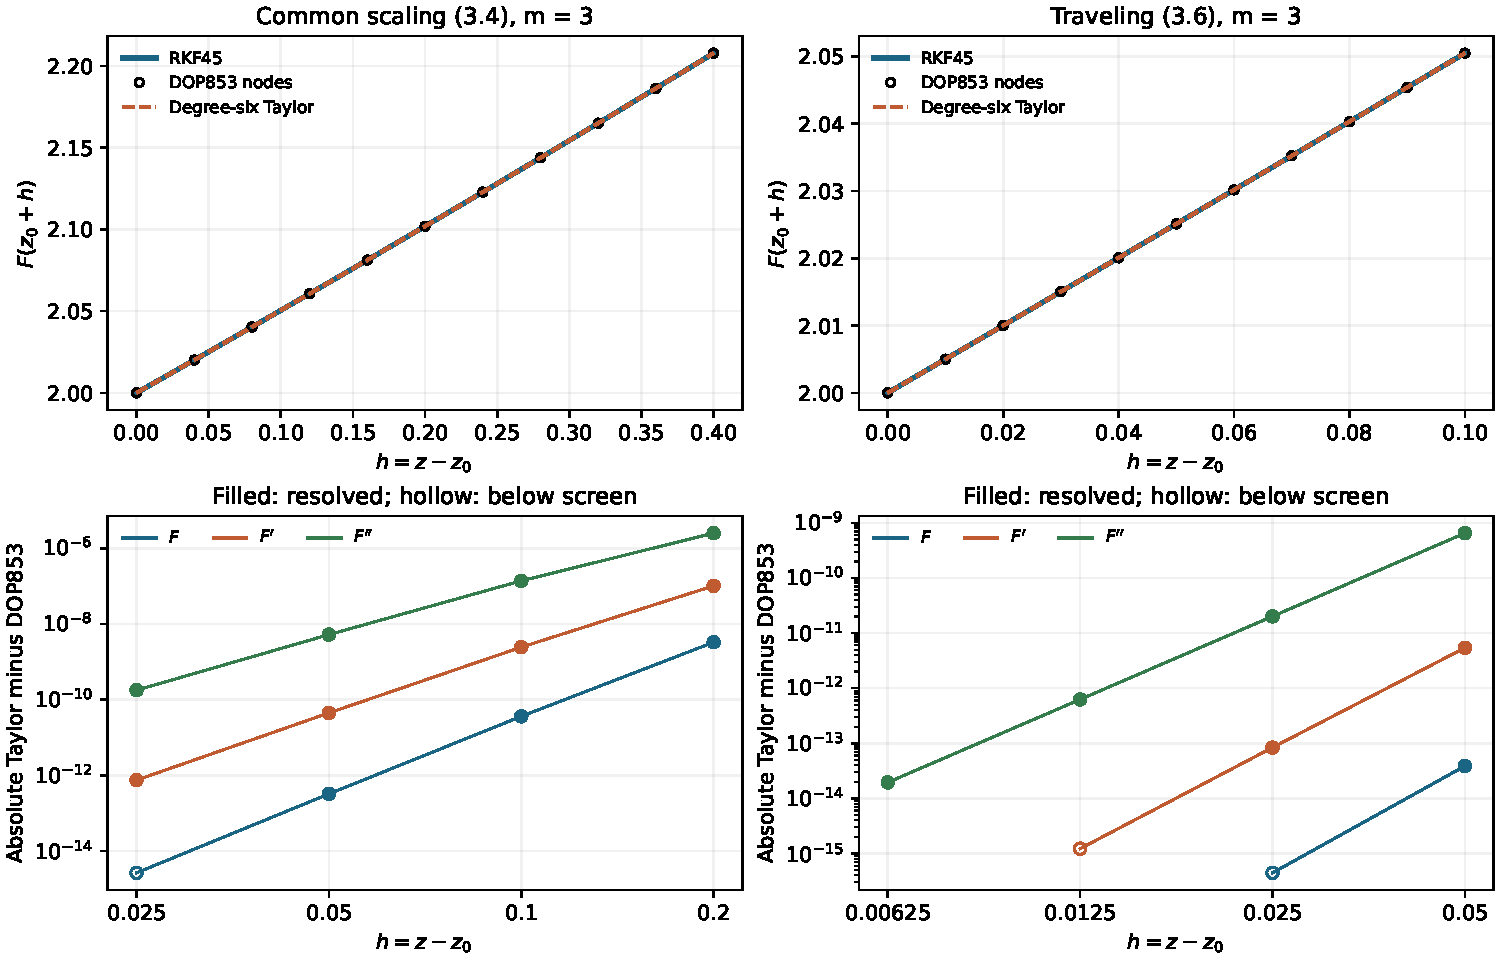
\includegraphics[width=\linewidth]{research_artifacts/SVE-reproduced-20261012/results/presentation/series-numerical.pdf}
\caption{Series and numerical views of the same constructed cubic IVPs.
Top: common-scaling (3.4) and traveling (3.6) profiles from RKF45, saved
DOP853 nodes and the degree-six Taylor polynomial; the curves overlap at
this scale. Bottom: separate absolute differences in $F,F',F''$ at four
saved nodes, without interpolation. Filled markers exceed the operational
resolution screen; hollow markers do not. Exact zero differences are omitted
from logarithmic axes. These finite differences show local truncation and
floating-resolution effects, not a certified remainder or a convergence
radius. Both panels use $(z_0,F_0,P_0,C_0)=(1,2,1/2,1/10)$,
$g=1$, $\kappa=1/30$, $m=3$; 3.6 uses $\alpha=-1$, $\alpha_3=0$.}
\label{fig:sve-series-numerical}
\end{figure}

\paragraph{Numerical method and independent comparisons.}
The numerical method is the classical six-stage embedded Fehlberg
4(5) pair~\cite{uddin2016rkf}. For the three-state system
$\boldsymbol y'=\boldsymbol f(z,\boldsymbol y)$ with
$\boldsymbol y=(F,P,C)$ and $\boldsymbol f=(P,C,R)$, a trial step
of length $\Delta z$ computes
\begin{align}
 \boldsymbol k_i&=\boldsymbol f\left(z_n+c_i\Delta z,
       \boldsymbol y_n+\Delta z\sum_{j<i}a_{ij}\boldsymbol k_j\right),
             \qquad i=1,\ldots,6,\notag\\
 \boldsymbol y_{n+1}^{(4)}&=\boldsymbol y_n+
                  \Delta z\sum_{i=1}^6b_i^{(4)}\boldsymbol k_i,\qquad
 \boldsymbol y_{n+1}^{(5)}=\boldsymbol y_n+
                  \Delta z\sum_{i=1}^6b_i^{(5)}\boldsymbol k_i.
 \label{eq:sve-rkf-step}
\end{align}
The coefficients are shown explicitly in Table~\ref{tab:sve-rkf-tableau};
thus the term ``RKF45'' specifies a method, not just a software label.
\begin{table}[htbp]
\centering\small
\begin{tabular}{@{}c|rrrrrr@{}}
\toprule
$c_i$ & \multicolumn{6}{c}{$a_{ij}$}\\
\midrule
$0$ & $0$ & & & & &\\
$1/4$ & $1/4$ & $0$ & & & &\\
$3/8$ & $3/32$ & $9/32$ & $0$ & & &\\
$12/13$ & $1932/2197$ & $-7200/2197$ & $7296/2197$ & $0$ & &\\
$1$ & $439/216$ & $-8$ & $3680/513$ & $-845/4104$ & $0$ &\\
$1/2$ & $-8/27$ & $2$ & $-3544/2565$ & $1859/4104$ & $-11/40$ & $0$\\
\midrule
$b^{(4)}$ & $25/216$ & $0$ & $1408/2565$ & $2197/4104$ & $-1/5$ & $0$\\
$b^{(5)}$ & $16/135$ & $0$ & $6656/12825$ & $28561/56430$ & $-9/50$ & $2/55$\\
\bottomrule
\end{tabular}
\caption{Classical Fehlberg embedded pair; blank stage entries are zero.}
\label{tab:sve-rkf-tableau}
\end{table}

The two approximations use the same six stage evaluations. Their difference
provides the local error indicator
\begin{equation}
 e=\left[\frac13\sum_{j=1}^3
 \left(\frac{y_{n+1,j}^{(5)}-y_{n+1,j}^{(4)}}
 {\mathrm{atol}+\mathrm{rtol}\max(|y_{n,j}|,|y_{n+1,j}^{(5)}|)}\right)^2
 \right]^{1/2}.
 \label{eq:sve-rkf-error}
\end{equation}
For $e\leq1$ the step is accepted and the fifth-order state is propagated;
otherwise the step is rejected and recomputed. For $e>0$ the proposed step
is multiplied by $\min(5,\max(0.2,0.9e^{-1/5}))$; when $e=0$ the
factor is $5$, subject to the same endpoint and maximum-step limits.
All stage evaluations must respect the positive-velocity, positive-gradient
and nonzero-leading-coefficient guards; a guard failure is not treated as
a valid continuation through a singularity. The defaults are
$\mathrm{rtol}=10^{-9}$, $\mathrm{atol}=10^{-11}$.

The reference for this choice uses Fehlberg with shooting for a
\emph{different} fluid boundary-value problem. It supplies neither the
constructed SVE initial data nor an SVE error guarantee. An eighth-order
Dormand--Prince method, DOP853, supplies an independent comparison;
the commonly named RK45 Dormand--Prince pair is not substituted for
Fehlberg's coefficients above.

All $21/21$ declared regular IVPs reached their endpoints under the
predeclared sampled gates. The maximum scaled Fehlberg--DOP853 state
disagreement was $1.09\times10^{-13}$; certified-integral drift, checked
only for 3.4, 3.6 and 3.9, was at most $7.33\times10^{-15}$.
The independent 3.4 two-state first-integral solve differed from the
three-state solve by at most $2.44\times10^{-15}$.
All five 3.8 rows agreed with their exact quadratic to at most
$4.44\times10^{-15}$. Coarse/fine Fehlberg solves had distinct accepted
time histories and endpoint differences at most $2.53\times10^{-10}$;
\emph{both} tolerance and maximum step were changed, so this is finite-step
consistency, not isolated tolerance convergence. Exact-quadratic differences
near roundoff are controls, not measured convergence orders.

\paragraph{First integrals as checks and as lower-order solvers.}
For the cubic 3.4, 3.6 and 3.9 IVPs, the exact initial constants are
$79/200$, $-71/200$ and $-79/200$, respectively. We evaluate
$I_4$ or $B(P)C$ on the saved three-state RKF45 trajectory. Separately,
we solve the two-state system obtained from that integral: use
$F'=P$, $P'=I_0/(I_4/C)$ in 3.4 and
\eqref{eq:sve-travel-two-state} in the traveling cases.
The initial $C_0$ is encoded in $I_0$, rather than silently dropped.
Figure~\ref{fig:sve-integral-checks} compares the resulting $(F,P)$ with the
third-order evolution. This tests a different differential formulation;
DOP853 supplies the second-order solve, so algebraic independence and
numerical-method comparison are both visible. These checks do not require
a variational Lagrangian. They are classical verified integrals, not learned
order-reducing discoveries, and no analogous certified integral is asserted
here for case 3.5.

\begin{figure}[htbp]
\centering
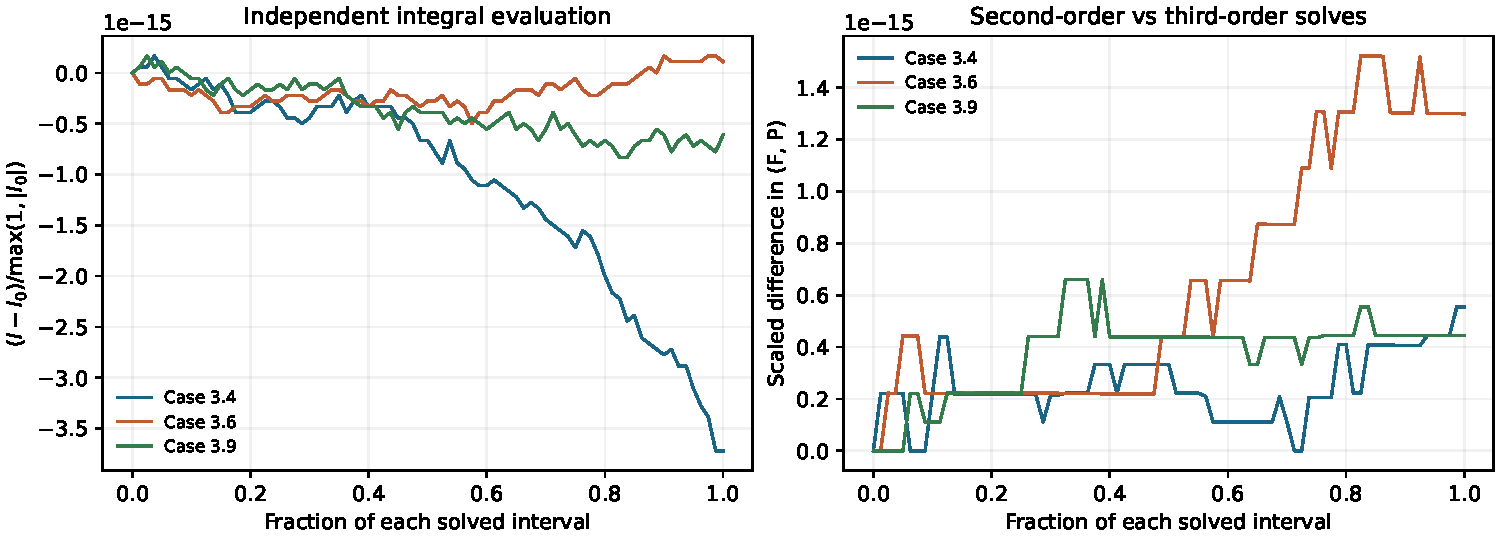
\includegraphics[width=\linewidth]{research_artifacts/SVE-reproduced-20261012/results/presentation/first-integral-checks.pdf}
\caption{Independent checks on the cubic common-scaling (3.4) and traveling
(3.6, 3.9) profiles. Left: signed integral drift relative to the exact
initial constant, scaled by $\max(1,|I_0|)$. Right: the maximum over the two
components $F,P$ of $|y_{\rm second}-y_{\rm third}|/\max(1,|y_{\rm third}|)$
at each saved node. The second-order equations use the fixed initial
integral; the third-order RKF45 equations do not enforce it. The horizontal
coordinate normalizes each solved interval, $[1,1.4]$ for 3.4 and $[1,1.1]$
for 3.6 and 3.9, for display only. Values near floating precision are
consistency diagnostics, not certified errors or measured convergence orders.}
\label{fig:sve-integral-checks}
\end{figure}

The original two-variable field was independently reconstructed and
differentiated by a nine-point tensor finite-difference stencil, without
substituting the ODE residual. At the declared $h=0.003$ stencil, the
largest original-PDE residuals were $7.98\times10^{-7}$ for a DOP853
reconstruction and $9.36\times10^{-7}$ for a tight-Fehlberg reconstruction,
both below the $10^{-6}$ gate. Finer $h=0.002,0.001$ probes are
roundoff-limited resolution diagnostics and often \emph{worsen}; they are
not convergence evidence. Sampled velocity and gradient stayed positive,
with minima $0.5$, and the smallest sampled absolute leading coefficient
was $1$. A $0.001t^3$ perturbation changed the checked PDE residual by at
least $0.00241$, a nonvacuity control. None of these finite samples proves
positivity between sample points, continuous residual bounds, global
accuracy, or compatibility with arbitrary initial-boundary data.

We measure convergence in two separate experiments.
Fixed-step Fehlberg runs with $N=1,2,4,8,16,32,64$ compare their endpoints
with a pair of tight DOP853 references; the exact quadratic replaces the
reference in 3.8. Pairwise orders are reported only when both errors exceed
an explicit reference/roundoff resolution screen. Of $147$ fixed-step errors,
$55$ are resolved and $92$ are below that threshold. The last resolved orders
are $4.97$--$4.98$ for the five 3.4 rows and $4.93$ for 3.5. Each short
traveling row yields only one resolved adjacent pair, around $4.95$--$4.97$;
this does not establish a sustained asymptotic range. The exact quadratic
has no measurable nontrivial order. An independent exact non-polynomial
control $y'=y$, $y(0)=1$ on $[0,2]$ approaches fifth order.

The adaptive sweep varies relative tolerance from $10^{-3}$ to $10^{-10}$,
with absolute tolerance one hundredth as large, fixed first-step and
maximum-step policies, and no forced output grid. Scaling-case endpoint
errors decrease from about $10^{-7}$ to $10^{-11}$ once the solver changes
its step history. The short traveling cases retain the same two steps and
show a tolerance plateau. The resolution screen is operational, not a
rigorous error bound. All $21$ cases complete both sweeps, with unresolved
orders retained whenever the reference precision is insufficient.


\subsection{Reconstructing the two-variable fields and the symbolic workflow}
After a profile has been found, the inverse substitution reconstructs a
field on the $(t,s)$ plane. This is what a two-dimensional profile plot
means here: time and \emph{one} material coordinate, not two spatial
coordinates. With normalized mass coordinate the particle position,
velocity and depth are
\[
 x_{\rm phys}=\phi(t,s),\qquad u(t,s)=\phi_t(t,s),\qquad
 h(t,s)=\frac1{\phi_s(t,s)}.
\]
The verified formulas give, for the admitted scaling graph,
\[
 \phi=t^AF(st^B),\qquad u=t^{A-1}(AF+BzF'),\qquad
 h=\frac{t^{-A-B}}{F'},\qquad z=st^B,
\]
and for a traveling graph,
\[
 \phi=\alpha_3t+F(s-\alpha t),\qquad
 u=\alpha_3-\alpha F',\qquad h=1/F'.
\]
These equations explain the shape and evolution of the reconstructed
surfaces. If a numerical profile is only known on $z\in[z_0,z_1]$,
only points whose invariant coordinate lies in that interval are
reconstructed. Extrapolation beyond it is not an additional solution.
The identifications are kinematic; the separate bed equations and their
compatibility still have to be checked before claiming a full physical SVE
solution.

The symbolic replication can now be described without reference to a
particular program interface. Algorithm~\ref{alg:sve-symbolic} specifies
the mathematical operations actually used. The source equations are
comparison inputs; the master equation supplies the reduced residuals.
The integration of determining equations and the adjoint-orbit arguments
are the mathematical deductions given above. They are not presented as
the output of an autonomous general-purpose classification algorithm.
\par\noindent\begin{minipage}{\linewidth}
\begin{algorithm}[Symbolic and numerical replication]
\label{alg:sve-symbolic}
\normalfont\small
\textbf{Input:} currents $\mathcal A,\mathcal J$; $g,\kappa>0$, $m\geq1$;
the chart $p,q>0$; printed formulas to compare; chosen initial data.
\begin{enumerate}
\item Define total derivatives on derivative coordinates through order three.
      Expand $E\gets D_t\mathcal A-gD_s\mathcal J$ and solve $E=0$ for $r$.
\item Introduce unrestricted $\tau(t,s,\phi),\xi(t,s,\phi),\eta(t,s,\phi)$.
      Set $Q\gets\eta-\tau p-\xi q$ and construct $\eta^I$ recursively.
\item Form $\Omega\gets\pr^{(3)}X(E)|_{r=\mathcal N}$.
      Extract the free-derivative coefficients in the stated order;
      integrate their equations separately at $m=1$, $m=3$, and $m\ne1,3$.
\item Substitute each resulting basis field into the full prolonged equation.
      Verify the off-shell multiplier identities, then compute brackets,
      adjoint actions and the stated line-equivalence cases.
\item For each selected generator, solve $X(z)=X(W)=0$ and set $W=F(z)$.
      Check $Q=0$ and the graph domain. Retain an explicit exceptional outcome
      if the graph fails or the master equation is undefined.
\item Differentiate each regular graph in the original variables through
      order three. Substitute into $E$ and factor the time or coordinate
      multiplier. Check this pullback against the compact current calculation.
\item For each analytically supplied candidate integral $I$, compute $DI$ and
      verify its equality to the stated reduced residual or multiplier.
      Record every denominator before solving for the highest derivative.
\item Compare the derived equations with the printed formulas by exact
      substitution. Preserve a counterexample whenever their residuals differ.
\item At each admissible initial jet, compute Taylor coefficients, verify
      the undivided residual, solve the ODE by Fehlberg's pair, and compare
      with the independent integrator and any lower-order integral equation.
\item Reconstruct $\phi,u,h$ only on the solved chart and independently
      differentiate the original two-variable field for a numerical check.
\end{enumerate}
\textbf{Output:} derived equations, generator and invariant tables,
parameter/graph restrictions, exact identities, source discrepancies,
and separately identified numerical diagnostics.
\end{algorithm}
\end{minipage}\par

For the nine numbered cases and declared numerical exponents, the
independent substitution route comprises 23 direct original-master checks
and two exceptional graph outcomes. It retains symbolic time in the
scaling factors. The adjoint comparison checks all 25 source Table 2
cells, and three first-integral identities are checked at symbolic $m$.
These exact calculations support the stated formulas; they are distinct
from the finite numerical convergence and residual experiments.
The scope throughout remains the local printed scalar equation.
